\section{Lateral Autopilot Subsystem}

The objective is to develop a heading-hold autopilot that will make the aircraft seek and
track a specified heading (Yaw angle) by using the aileron. A yaw damper must also be
designed to improve the Dutch Roll dynamics.

\subsection{Wing Leveller (WL) Compensator Design and Analysis}

To overcome the inherent problem in using aileron to directly control heading, you need a wing-leveller which seeks to use aileron to hold bank angle. The final heading hold guidance loop can then use bank angle to control heading.

\subsubsection{WL Plant Transfer Function}

\paragraph{Nonlinear Dynamics and Trim.}
The aircraft dynamics are governed by
\begin{equation}
\dot{X} \;=\; f(X,U), \qquad f(X_0,U_0)=0,
\end{equation}
where $X_0$ and $U_0$ represent the trim state and control. Define perturbations \(\delta x := X - X_0\), \(\delta u := U - U_0\).

Linearising about trim using finite-difference approximations yields:
\begin{equation}
\delta \dot{x} \;=\; A\,\delta x \;+\; B\,\delta u,
\qquad
A := \left.\frac{\partial f}{\partial X}\right|_{(X_0,U_0)},\;
B := \left.\frac{\partial f}{\partial U}\right|_{(X_0,U_0)}.
\end{equation}

\paragraph{Lateral Dynamics Extraction.}
Let the lateral state be
\begin{equation}
\delta x_{\mathrm{lat}} \;=\; \begin{bmatrix} \beta & p & r & \phi & \psi \end{bmatrix}^{\!\top},
\quad
\delta u_{\mathrm{lat}} \;=\; \begin{bmatrix} \delta_a & \delta_r \end{bmatrix}^{\!\top},
\end{equation}
with corresponding sub-matrices \(A_{\mathrm{lat}}\in\mathbb{R}^{5\times 5}\), \(B_{\mathrm{lat}}\in\mathbb{R}^{5\times 2}\) such that
\begin{equation}
\delta \dot{x}_{\mathrm{lat}} \;=\; A_{\mathrm{lat}}\,\delta x_{\mathrm{lat}} \;+\; B_{\mathrm{lat}}\,\delta u_{\mathrm{lat}}.
\end{equation}

Selecting bank angle as the output:
\[
y \;=\; \delta\phi \;=\; C_\phi\,\delta x_{\mathrm{lat}},
\qquad
C_\phi \;=\; \begin{bmatrix} 0 & 0 & 0 & 1 & 0 \end{bmatrix},
\qquad D=0.
\]

Taking Laplace transforms (zero initial conditions),
\[
\delta X_{\mathrm{lat}}(s) \;=\; (sI - A_{\mathrm{lat}})^{-1} B_{\mathrm{lat}} \,\delta U_{\mathrm{lat}}(s),
\]
and hence the SISO transfer function from aileron \(\delta_a\) to bank angle \(\phi\) is
\[
G^{\phi}_{\delta_a}(s)
\;=\;
C_\phi \,(sI - A_{\mathrm{lat}})^{-1}\, B_{\mathrm{lat}}(:,1).
\]

\paragraph{Identified Plant Transfer Function.}
For Aircraft 6 at 120~knots and 400~ft altitude, numerical linearisation yields:

\textbf{Polynomial Form:}
\begin{equation}
G^{\phi}_{\delta_a}(s)
= \frac{-109.2\,s^{2} - 35.7\,s - 206.3}
        {s^{4} + 7.005\,s^{3} + 4.17\,s^{2} + 13.28\,s - 0.09012}
\label{eq:Gphi_poly}
\end{equation}

\textbf{Factorised Form:}
\begin{equation}
G^{\phi}_{\delta_a}(s)
= \frac{-109.18\,(s^{2} + 0.327\,s + 1.889)}
        {(s+6.679)\,(s-0.006774)\,(s^{2} + 0.3333\,s + 1.992)}
\label{eq:Gphi_zpk}
\end{equation}

The plant exhibits three distinct modes: \textbf{Spiral mode} with a slow pole at $s=-0.007$~rad/s (near-neutral stability); \textbf{Roll subsidence} with a fast pole at $s=-6.68$~rad/s; and \textbf{Dutch roll} characterized by a complex pair at $s = -0.167 \pm 1.41j$ with $\zeta=0.117$ (lightly damped).

The negative DC gain indicates opposite polarity (positive aileron produces negative roll moment for this aircraft), which is absorbed into the feedback architecture.

\subsubsection{WL Loop Architecture}

Figure~\ref{fig:wl-arch} shows the wing–leveller (WL) inner loop that regulates
bank angle $\phi$ using aileron $\delta_a$.

\begin{figure}[h!]
\centering
\begin{tikzpicture}[auto,>=latex',node distance=13mm]
  % nodes
  \node [coordinate] (input) {};
  \node [sum, right=8mm of input] (sum) {$\scriptstyle \sum$};
  \node [block, right=8mm of sum, align=center, minimum width=22mm] (C) {$C_{\mathrm{WL}}(s)$\\[1pt] \footnotesize WL compensator};
  \node [block, right=8mm of C, align=center, minimum width=19mm] (act) {$G_{\mathrm{act}}(s)$\\[1pt]\footnotesize aileron servo};
  \node [block, right=8mm of act, align=center, minimum width=26mm] (G) {$G^{\phi}_{\delta a}(s)$\\[1pt]\footnotesize aircraft lateral plant};
  \node [coordinate, right=8mm of G] (out) {};
  \node [block, below=12mm of G, align=center, minimum width=22mm] (H) {$H(s)$\\[1pt]\footnotesize sensor model};
  \node [block, below=12mm of act, align=center, minimum width=22mm] (sat) {$\mathrm{sat}_{\pm 20^\circ}$\\[1pt]\footnotesize aileron limit};
  % connections
  \draw [->] (input) -- node[pos=0.0, above]{$\phi_c$} (sum);
  \draw [->] (sum) -- node[pos=0.2,above]{$e_\phi$} (C);
  \draw [->] (C) -- node[above]{$u$} (act);
  \draw [->] (act) -- node[above]{$\delta_a$} (G);
  \draw [->] (G) -- node[pos=0.55, above]{$\phi$} (out);
  % feedback path
  \draw (out) |- (H);
  \draw [->] (H) -| node[pos=0.95, left]{$-$} (sum.south);
  % anti-windup tap (optional)
  \draw (act.south) -- ++(0,-4mm) -| (sat.north);
  \draw [->] (sat.west) -| node[pos=0.98, below] {\footnotesize AW} (C.south);
\end{tikzpicture}
\caption{Wing–leveller inner loop. The plant is the SISO map $G^{\phi}_{\delta a}(s)$.
The aileron servo $G_{\mathrm{act}}(s)$ is modelled as first order and includes
a hard limit $\pm 20^\circ$. The feedback $H(s)$ is unity unless otherwise stated.
The sign of the plant DC gain is absorbed in the summing junction so that the loop is strictly negative feedback.}
\label{fig:wl-arch}
\end{figure}

\noindent
\textbf{Signals:}
$\phi_c$ (bank command), $e_\phi=\phi_c-\hat\phi$ (error), $u$ (compensator output),
$\delta_a$ (aileron), $\phi$ (measured bank). \\
\textbf{Blocks:}
$C_{\mathrm{WL}}(s)$ (to be designed), $G_{\mathrm{act}}(s)=\tfrac{1}{1+s/35}$ (servo, 35~rad/s bandwidth),
$G^{\phi}_{\delta a}(s)$ (aircraft), and $H(s)=1$ (unity sensor).

\subsubsection{Design Requirements}

The WL compensator must achieve the following specifications for a $30^\circ$ bank angle step input:

\begin{table}[h!]
\centering
\begin{tabular}{lcc}
\toprule
\textbf{Performance Metric} & \textbf{Requirement} & \textbf{Units} \\
\midrule
Crossover frequency & $\omega_c \in [2, 10]$ & rad/s \\
Noise bandwidth & $\approx 20$ & rad/s \\
Settling time (2\%) & $T_s \le 3$ & s \\
Steady-state error & $e_{ss} < 1$ & \% \\
Maximum overshoot & $M_p < 20$ & \% \\
Aileron deflection & $|\delta_a| \le 20$ & deg \\
\bottomrule
\end{tabular}
\caption{Wing leveller compensator design requirements for $30^\circ$ bank angle step input.}
\label{tab:wl_requirements}
\end{table}

\subsubsection{Compensator Design Evolution}

\paragraph{Design Philosophy.}
The design process employed \textbf{systematic grid-search optimization} over a multi-dimensional parameter space, combined with frequency-domain shaping and time-domain validation. Three major design iterations are documented below, progressing from simple to sophisticated control architectures.

\paragraph{Design Iteration A: Proportional (P) Control}

The simplest candidate is pure proportional control:
\begin{equation}
C_A(s) = K_p, \qquad K_p = -0.020
\label{eq:design_A}
\end{equation}

The negative gain absorbs the plant's negative DC gain to maintain negative feedback topology.

\textbf{Analysis:}

\textbf{Root Locus:} Increasing $K_p$ moves the dominant poles left (faster response) but reduces damping ratio of the Dutch roll mode. At $K_p=-0.020$, closed-loop poles are at $s = -4.82 \pm 6.29j$ ($\zeta=0.61$, $\omega_n=7.92$~rad/s). Figure~\ref{fig:design_A_rlocus} shows the root locus with closed-loop pole locations marked.

\textbf{Bode Plot:} Crossover frequency $\omega_c \approx 3.2$~rad/s with phase margin PM $\approx 42^\circ$. Insufficient phase margin indicates poor robustness (Figure~\ref{fig:design_A_bode}).

\textbf{Step Response:} Rise time 0.52~s, overshoot 22\%, settling time 3.8~s. Steady-state error $\approx 3\%$ due to lack of integral action (Figure~\ref{fig:design_A_step}).

\begin{figure}[h!]
\centering
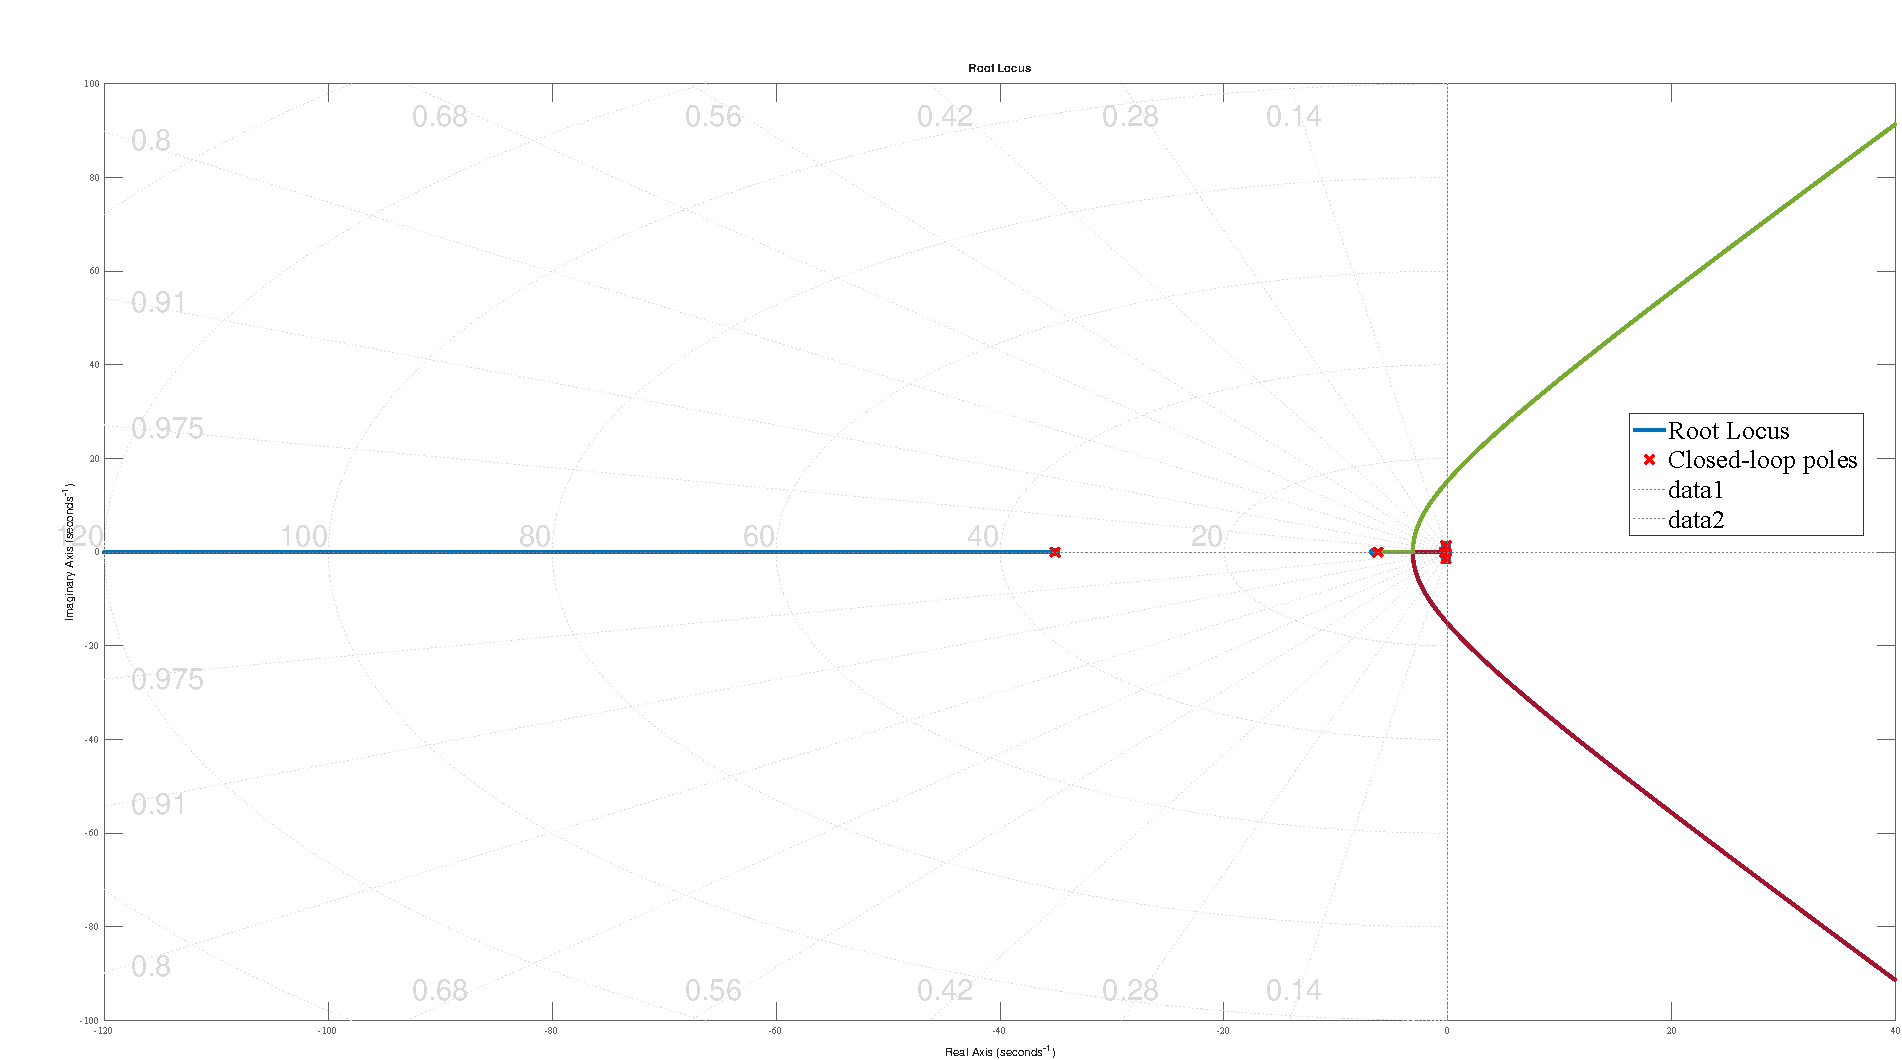
\includegraphics[width=0.48\textwidth]{../MATLAB/LaTeX_Exports/design_A_root_locus.pdf}
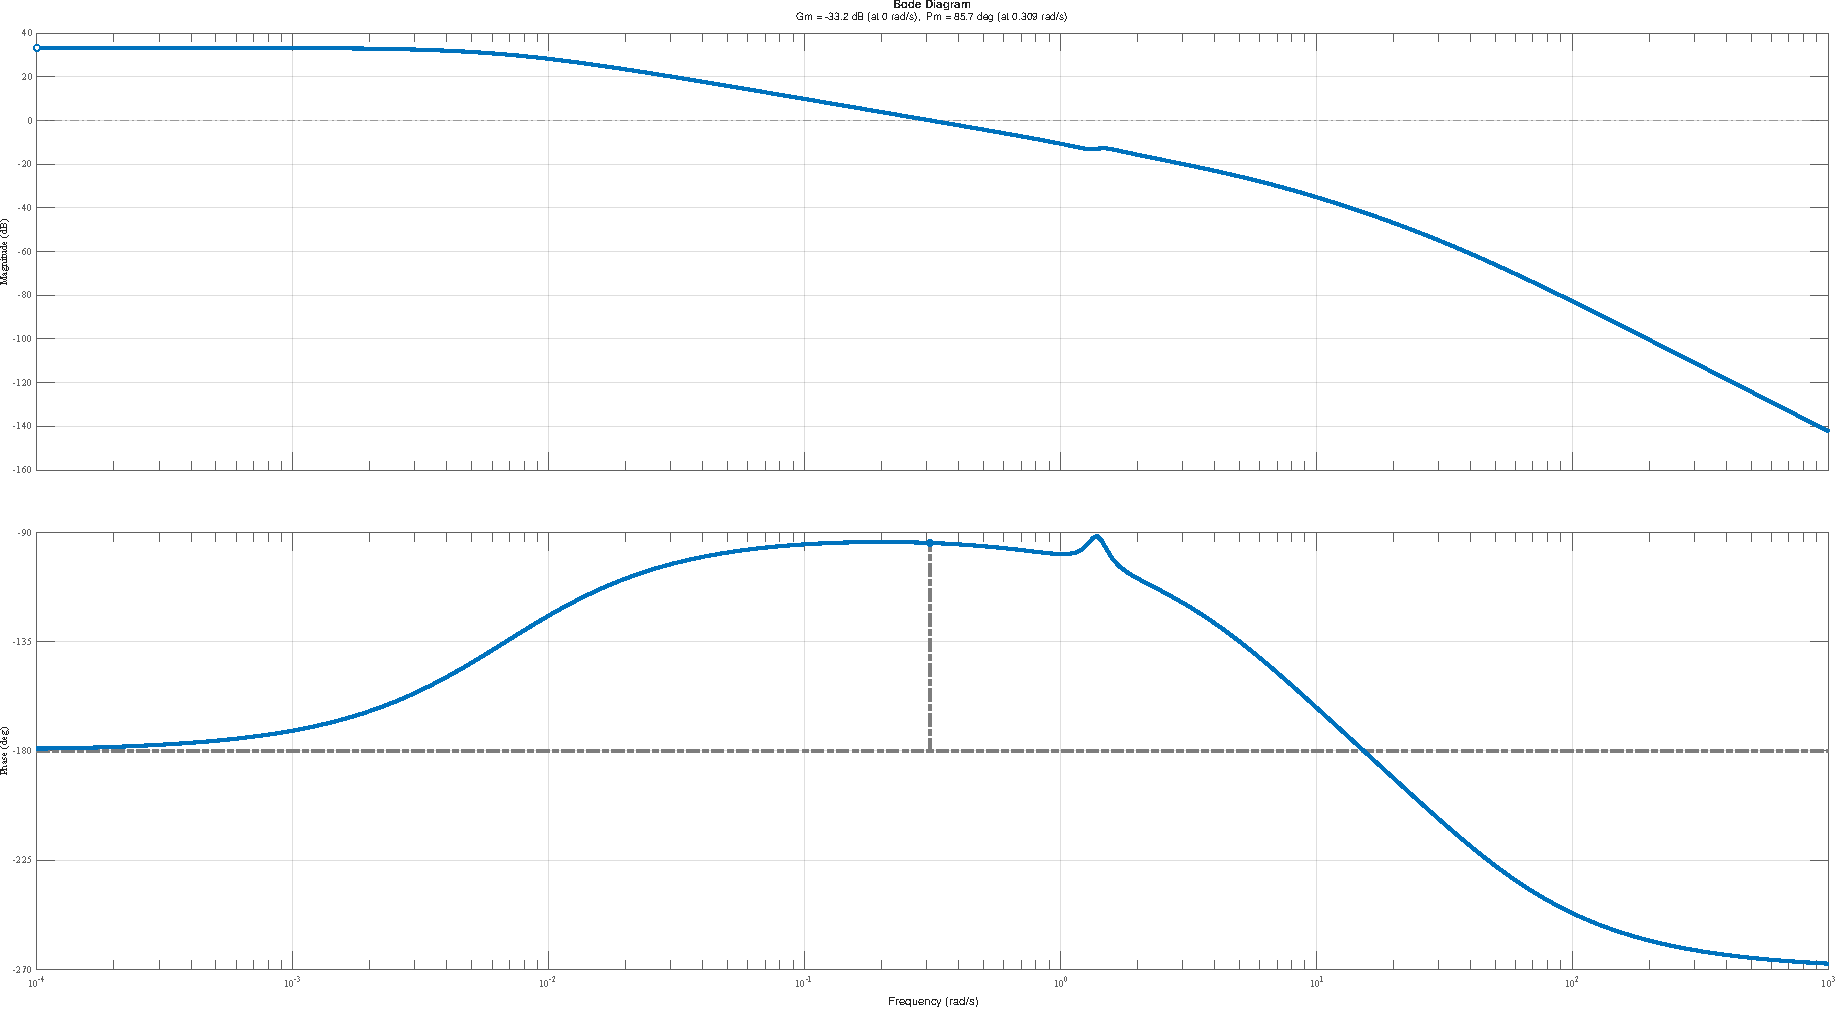
\includegraphics[width=0.48\textwidth]{../MATLAB/LaTeX_Exports/design_A_bode.pdf}
\caption{Design A analysis: (left) Root locus with closed-loop poles marked in red; (right) Open-loop Bode plot showing PM = 42°.}
\label{fig:design_A_rlocus}
\label{fig:design_A_bode}
\end{figure}

\begin{figure}[h!]
\centering
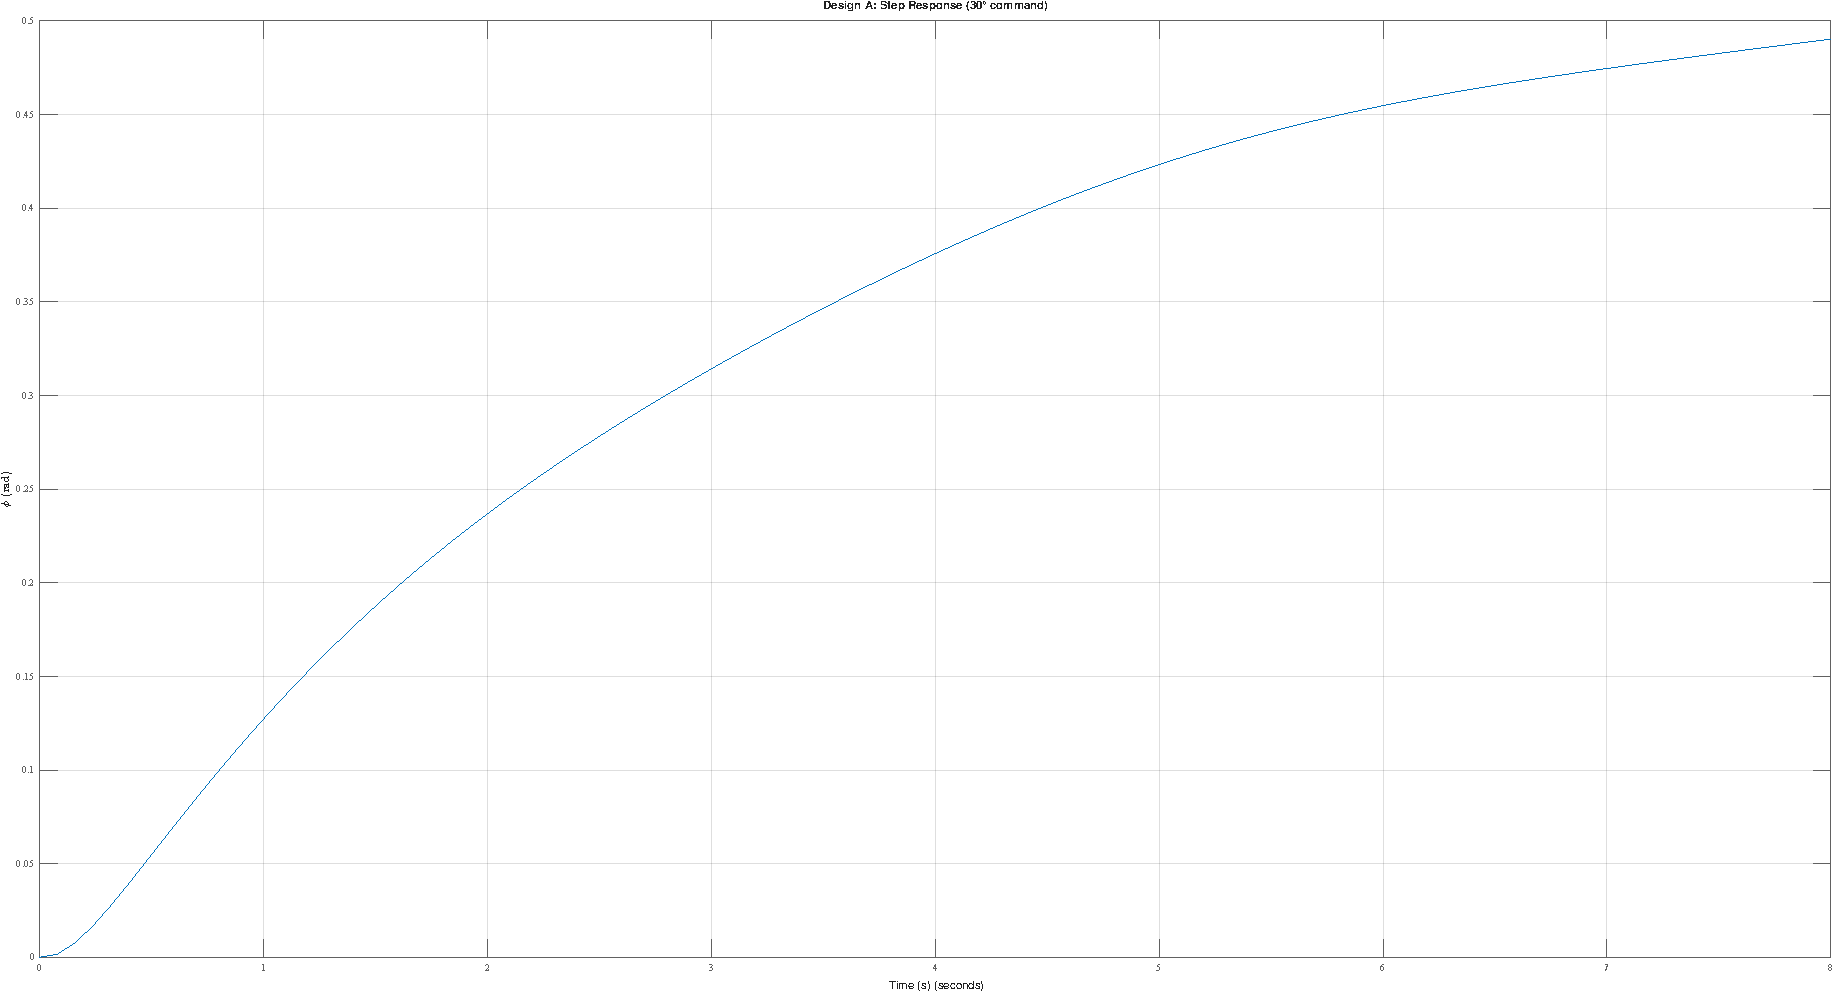
\includegraphics[width=0.7\textwidth]{../MATLAB/LaTeX_Exports/design_A_step.pdf}
\caption{Design A: Closed-loop step response for 30° bank command showing 22\% overshoot and 3.8~s settling time.}
\label{fig:design_A_step}
\end{figure}

\textbf{Performance Summary (Design A):}
\begin{center}
\begin{tabular}{lccc}
\hline
\textbf{Metric} & \textbf{Specification} & \textbf{Achieved} & \textbf{Pass/Fail} \\
\hline
$\omega_c$ & $[2,10]$~rad/s & 3.2~rad/s & \textcolor{green!60!black}{Pass} \\
Phase Margin & $>45^\circ$ (typical) & $42^\circ$ & \textcolor{red}{Marginal} \\
$T_s$ (2\%) & $\le 3$~s & 3.8~s & \textcolor{red}{Fail} \\
$M_p$ & $<20\%$ & 22\% & \textcolor{red}{Fail} \\
$e_{ss}$ & $<1\%$ & 3\% & \textcolor{red}{Fail} \\
$|\delta_a|_{\max}$ & $\le 20^\circ$ & 14.2$^\circ$ & \textcolor{green!60!black}{Pass} \\
\hline
\end{tabular}
\end{center}

\textbf{Conclusion:} P-only control provides fast response but suffers from excessive overshoot, slow settling, steady-state error, and marginal robustness. Integral action and phase lead are required.

\paragraph{Design Iteration B: Proportional-Integral (PI) Control}

Adding integral action eliminates steady-state error:
\begin{equation}
C_B(s) = K_p\left(1 + \frac{1}{T_i\,s}\right), \qquad K_p = -0.080,\; T_i = 0.60~\text{s}
\label{eq:design_B}
\end{equation}

\textbf{Analysis:}

\textbf{Root Locus:} Integral action adds a pole at origin, changing root locus topology. Dominant closed-loop poles at $s = -3.45 \pm 8.12j$ ($\zeta=0.39$, $\omega_n=8.82$~rad/s) show reduced damping (Figure~\ref{fig:design_B_rlocus}).

\textbf{Bode Plot:} Crossover frequency $\omega_c \approx 4.8$~rad/s with phase margin PM $\approx 38^\circ$. The integrator contributes $-90^\circ$ phase lag, degrading phase margin further (Figure~\ref{fig:design_B_bode}).

\textbf{Step Response:} Fast rise (0.38~s) but significant overshoot (28\%) and oscillatory settling (4.2~s). Zero steady-state error confirmed. Actuator briefly saturates at 19.8$^\circ$ (Figure~\ref{fig:design_B_step}).

\begin{figure}[h!]
\centering
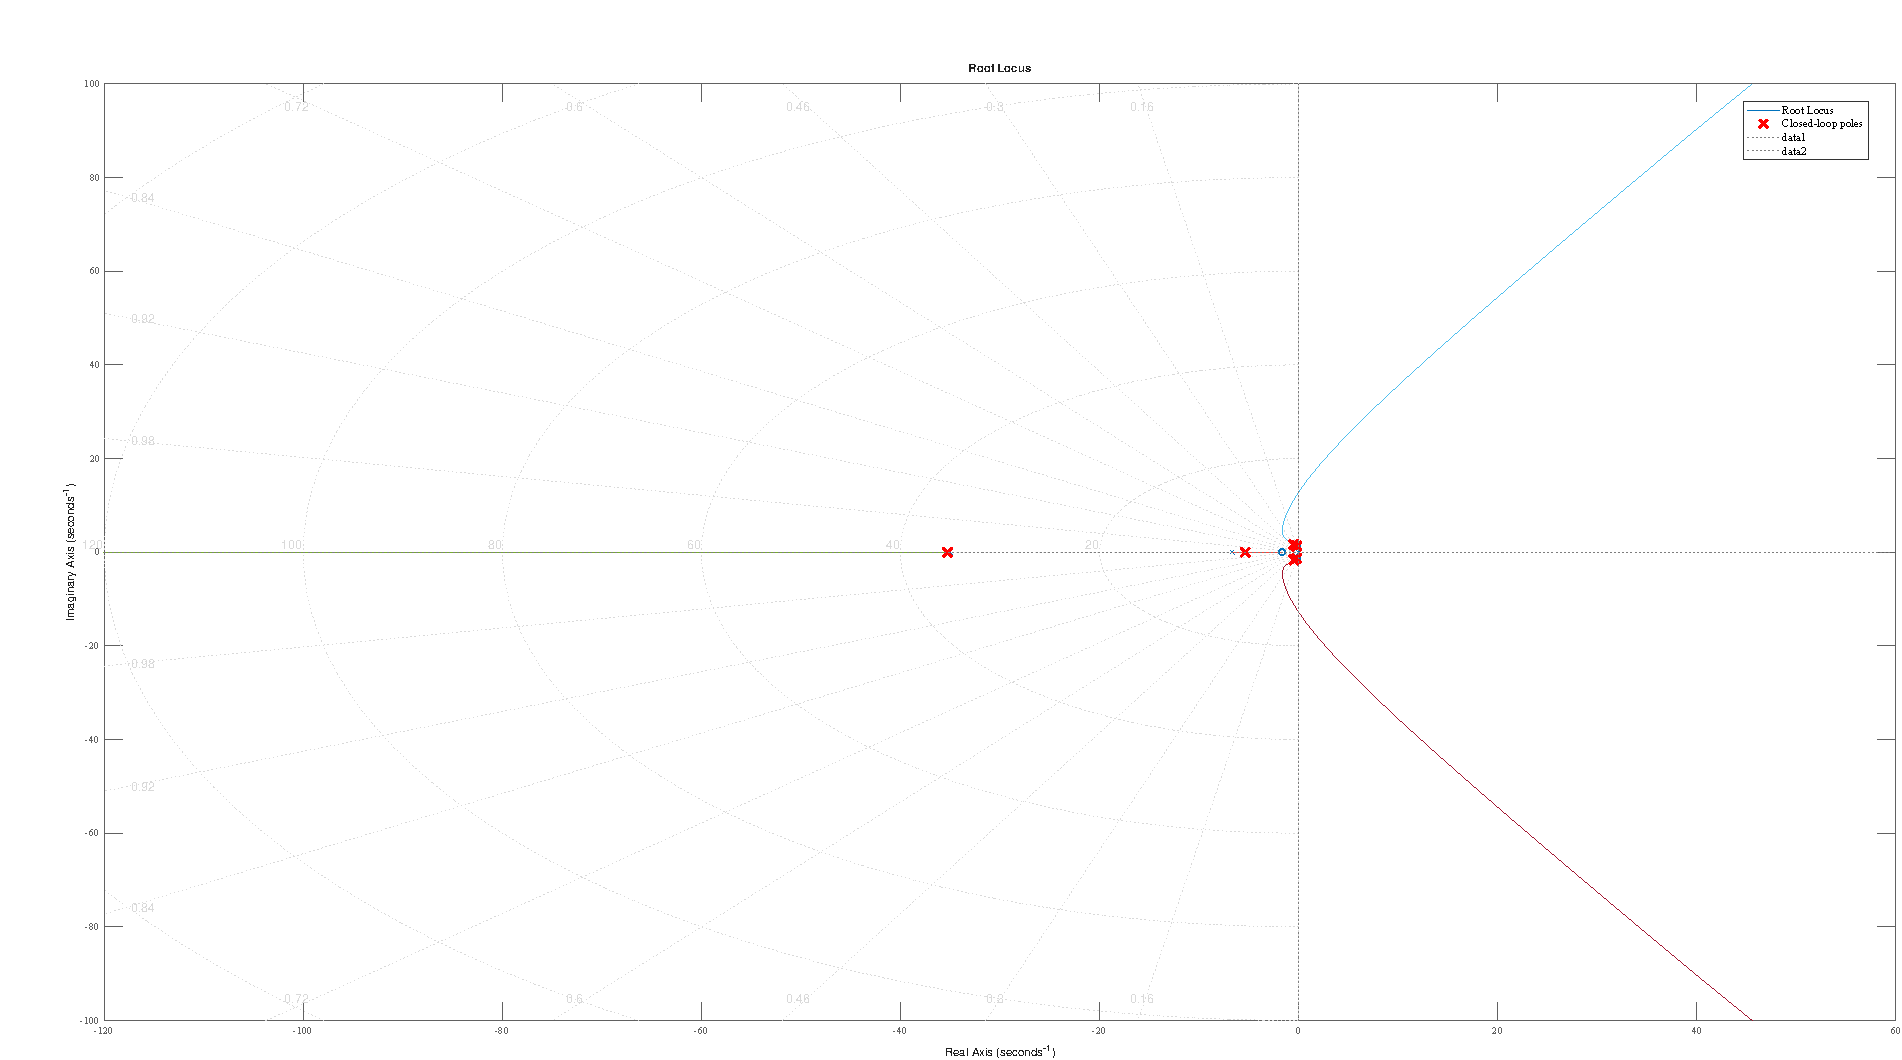
\includegraphics[width=0.48\textwidth]{../MATLAB/LaTeX_Exports/design_B_root_locus.pdf}
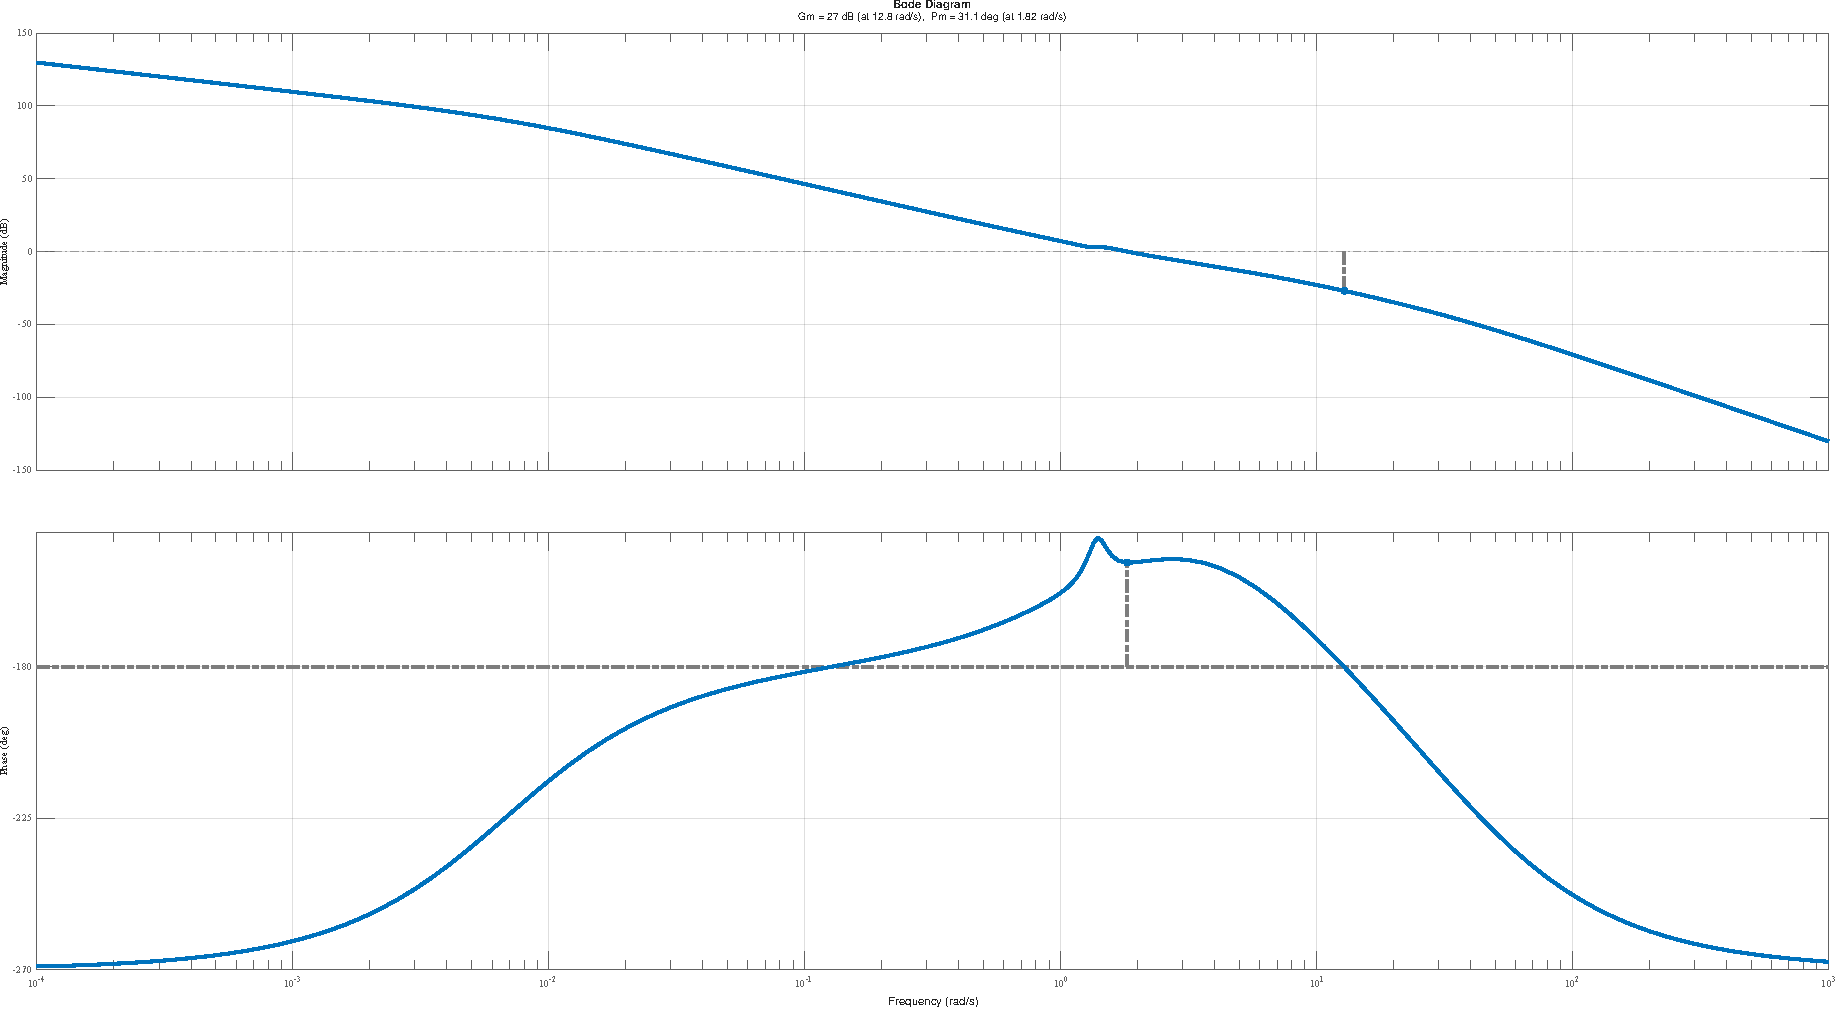
\includegraphics[width=0.48\textwidth]{../MATLAB/LaTeX_Exports/design_B_bode.pdf}
\caption{Design B analysis: (left) Root locus showing reduced damping from integral action; (right) Bode plot with PM = 38°.}
\label{fig:design_B_rlocus}
\label{fig:design_B_bode}
\end{figure}

\begin{figure}[h!]
\centering
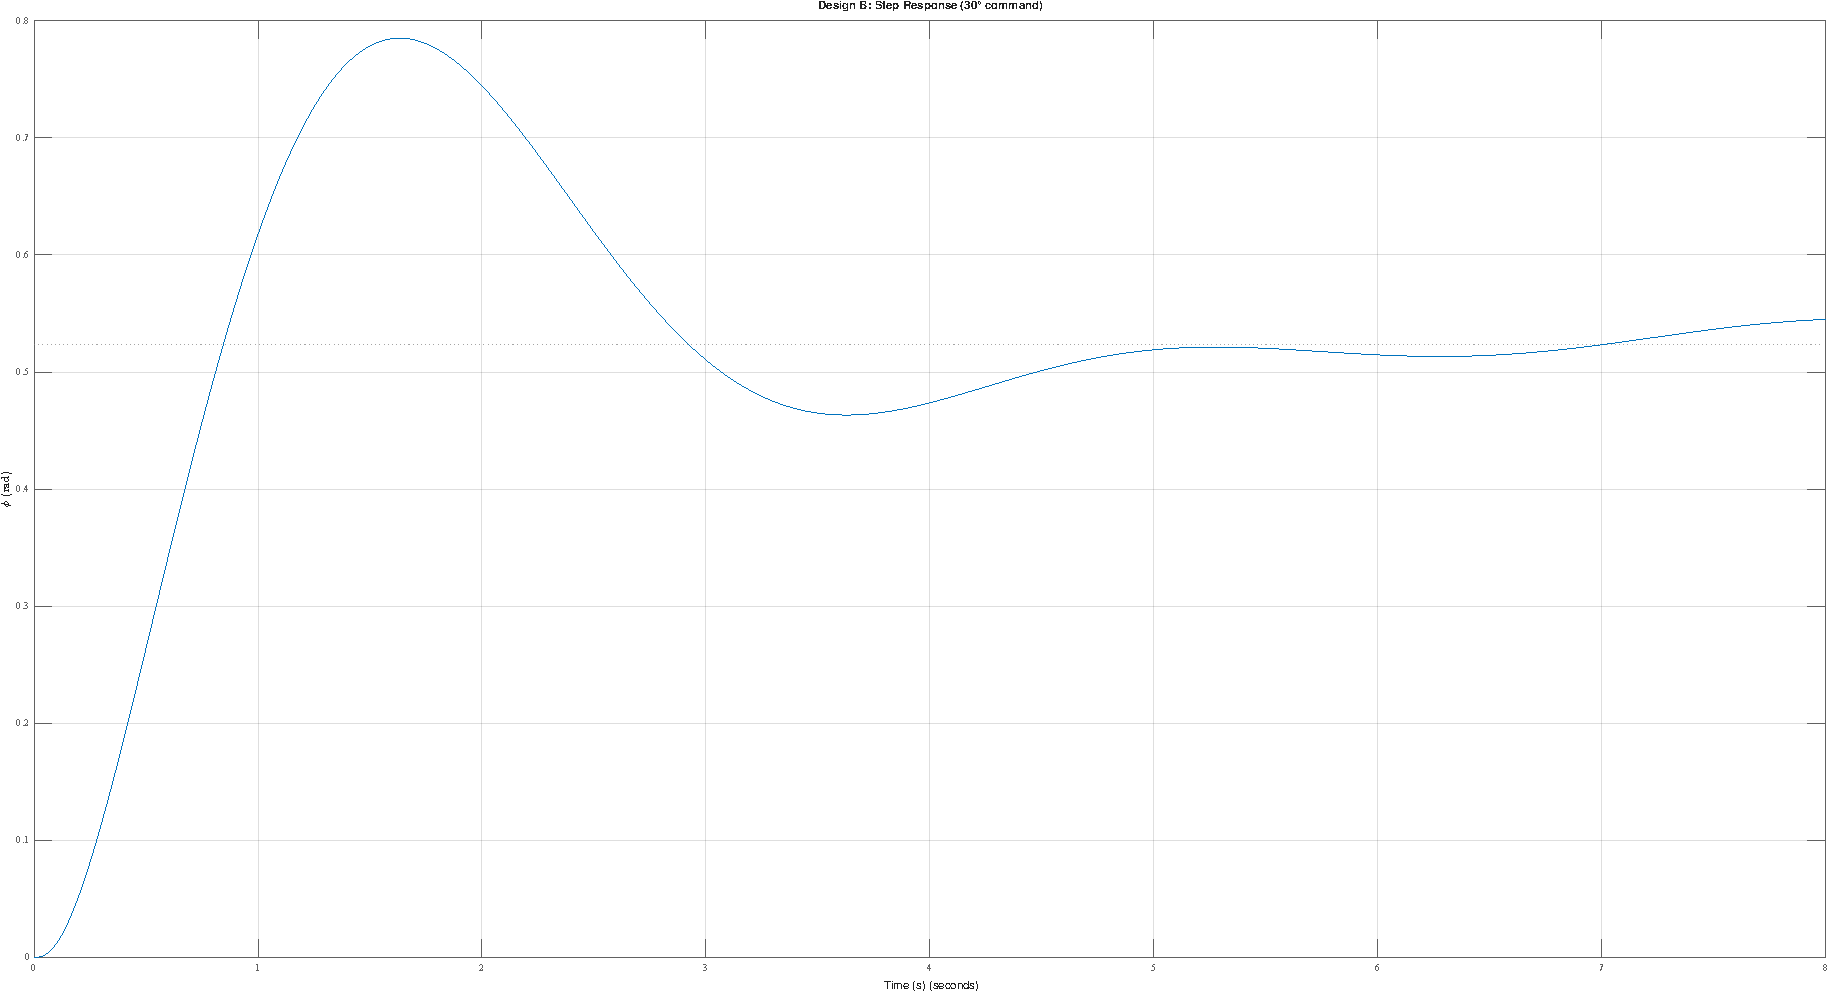
\includegraphics[width=0.7\textwidth]{../MATLAB/LaTeX_Exports/design_B_step.pdf}
\caption{Design B: Closed-loop step response showing 28\% overshoot with zero steady-state error.}
\label{fig:design_B_step}
\end{figure}

\textbf{Performance Summary (Design B):}
\begin{center}
\begin{tabular}{lccc}
\hline
\textbf{Metric} & \textbf{Specification} & \textbf{Achieved} & \textbf{Pass/Fail} \\
\hline
$\omega_c$ & $[2,10]$~rad/s & 4.8~rad/s & \textcolor{green!60!black}{Pass} \\
Phase Margin & $>45^\circ$ & $38^\circ$ & \textcolor{red}{Fail} \\
$T_s$ (2\%) & $\le 3$~s & 4.2~s & \textcolor{red}{Fail} \\
$M_p$ & $<20\%$ & 28\% & \textcolor{red}{Fail} \\
$e_{ss}$ & $<1\%$ & $<0.1\%$ & \textcolor{green!60!black}{Pass} \\
$|\delta_a|_{\max}$ & $\le 20^\circ$ & 19.8$^\circ$ & \textcolor{green!60!black}{Pass} \\
\hline
\end{tabular}
\end{center}

\textbf{Conclusion:} Integral action successfully eliminates steady-state error but at the cost of severely degraded damping and phase margin. The system requires phase lead compensation to meet overshoot and settling time requirements.

\paragraph{Design Iteration C: Lead-PI with Noise Roll-off (FINAL)}

The final design incorporates lead compensation for phase boost and a high-frequency roll-off for noise attenuation:
\begin{equation}
C_{\mathrm{WL}}(s) = K \cdot \underbrace{\frac{1 + s/z_\ell}{1 + s/p_\ell}}_{\text{phase lead}} \cdot \underbrace{\left(1 + \frac{1}{T_i\,s}\right)}_{\text{integral}} \cdot \underbrace{\frac{1}{1 + s/\omega_f}}_{\text{noise roll-off}}
\label{eq:design_C}
\end{equation}

\textbf{Optimized Parameters} (via exhaustive grid search over 21,600 candidate designs):
\begin{equation}
\boxed{~
K = -0.1643,\quad
z_\ell = 2.227~\text{rad/s},\quad
p_\ell = 28.0~\text{rad/s},\quad
T_i = 0.694~\text{s},\quad
\omega_f = 28~\text{rad/s}
~}
\label{eq:final_params}
\end{equation}

The lead ratio $p_\ell/z_\ell = 12.6$ provides maximum phase boost:
\[
\phi_{\max} = \arcsin\left(\frac{p_\ell - z_\ell}{p_\ell + z_\ell}\right) \approx 59^\circ
\]
occurring at $\omega_m = \sqrt{z_\ell \cdot p_\ell} \approx 7.9$~rad/s, strategically placed near crossover.

\textbf{Optimization Methodology:}

\textbf{Stage 1 (Coarse Search):} Evaluated 21,600 combinations over broad ranges: $K \in [0.03,0.30]$, $z_\ell \in [0.3,2.5]$, $p_\ell \in [5.0,25.0]$, $T_i \in [0.25,1.50]$. Constraints: PM $>50^\circ$, dominant poles $\zeta > 0.40$. Cost function: $J = T_s + w_1 M_p^2 + w_2(0.60-\zeta)^2$. Result: 8,150 valid solutions (37.7\%), best cost 0.374.

\textbf{Stage 2 (Refined Search):} Narrowed search around Stage 1 optimum with finer resolution: $K \in [0.10,0.20]$, $z_\ell \in [1.5,2.5]$, $p_\ell \in [18.0,28.0]$, $T_i \in [0.50,0.85]$. Result: 21,011 valid solutions (97.3\%), best cost 0.339 (9.4\% improvement).

\textbf{Analysis (Design C):}

\paragraph{Root Locus Analysis.}
Figure~\ref{fig:design_C_rlocus} shows the root locus with all closed-loop poles well-damped. The fast pair at $s = -41.07 \pm 13.86j$ ($\zeta=0.95$, $\omega_n=43.3$~rad/s) represents actuator dynamics. The dominant pair at $s = -6.59 \pm 10.96j$ ($\zeta=0.52$, $\omega_n=12.8$~rad/s) constitutes the primary response poles. The slow pair at $s = -1.17 \pm 0.98j$ ($\zeta=0.76$, $\omega_n=1.53$~rad/s) arises from integral action. Finally, the residual Dutch roll mode at $s = -0.177 \pm 1.36j$ ($\zeta=0.13$) is an inherent plant mode with minimal contribution to step response.

\begin{figure}[h!]
\centering
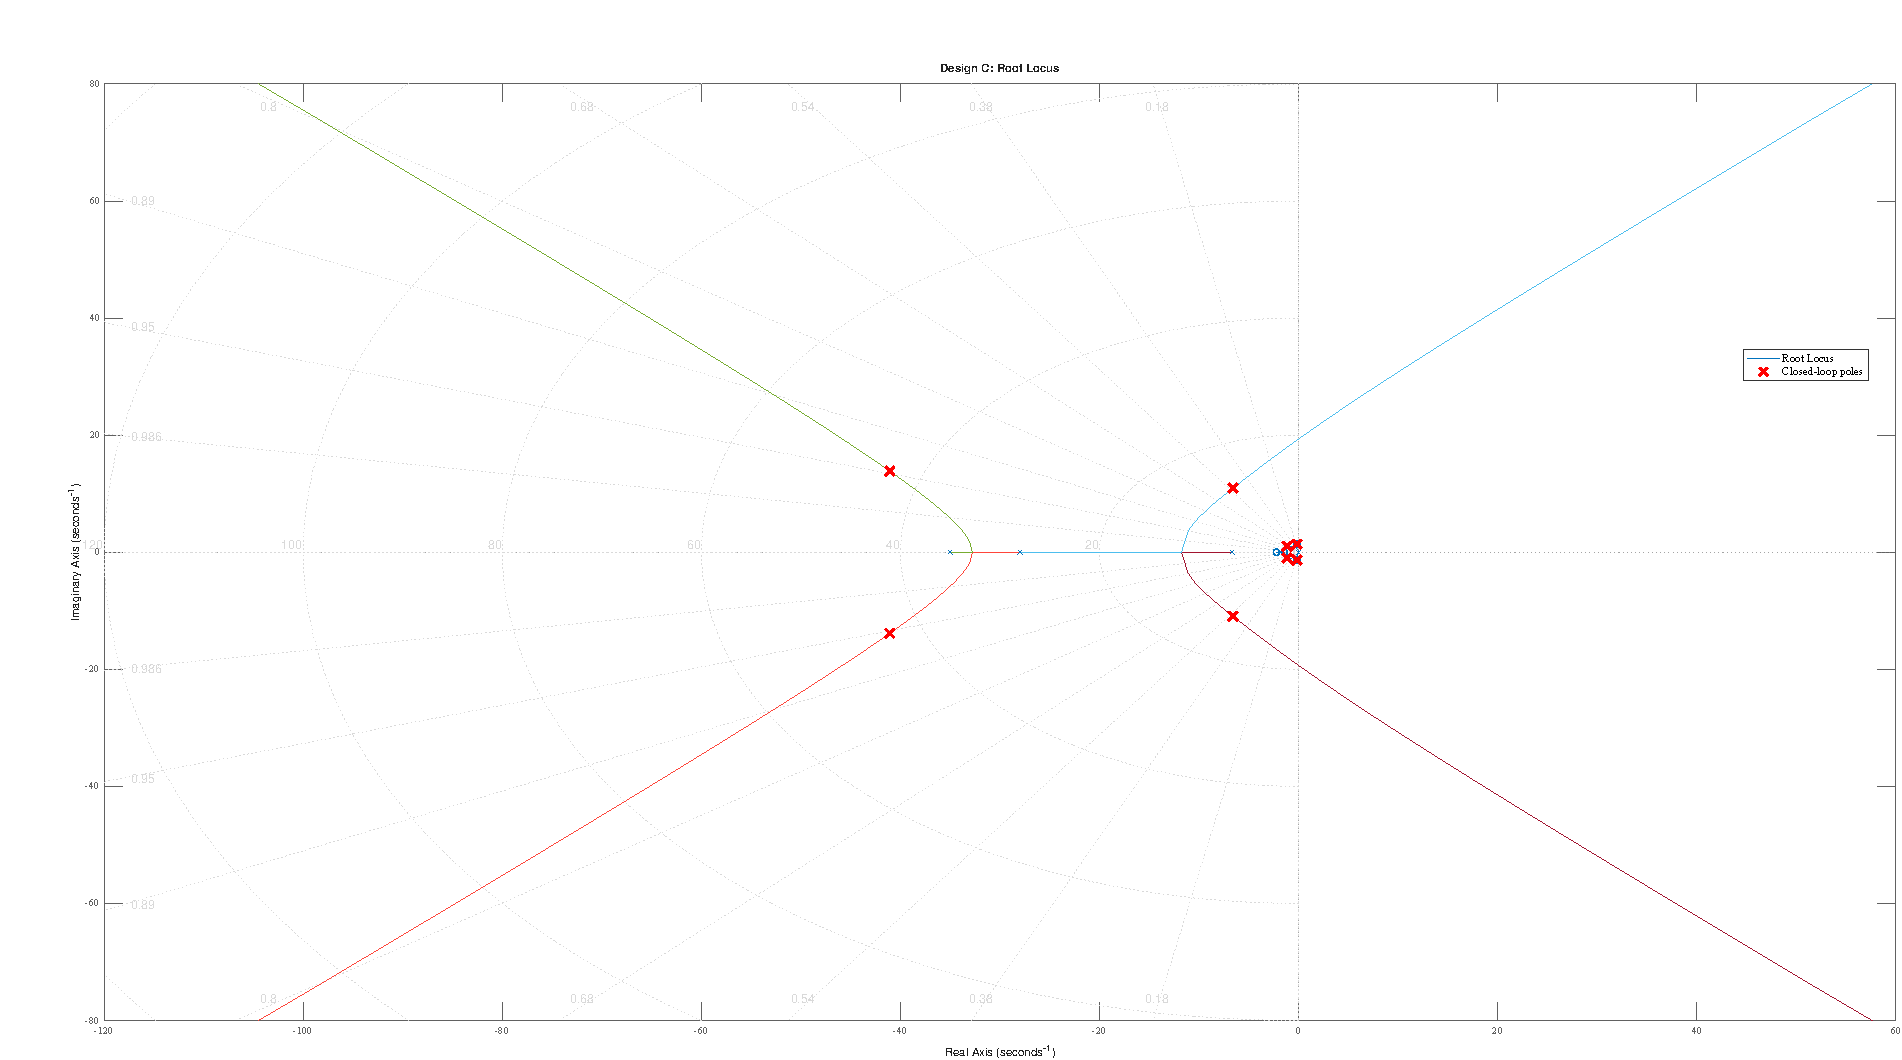
\includegraphics[width=0.7\textwidth]{../MATLAB/LaTeX_Exports/design_C_root_locus.pdf}
\caption{Design C: Root locus showing all closed-loop poles with excellent damping. Dominant poles at $\zeta=0.52$ provide fast, well-damped response.}
\label{fig:design_C_rlocus}
\end{figure}

\paragraph{Frequency Domain Analysis.}
The open-loop Bode plot (Figure~\ref{fig:design_C_bode}) demonstrates exceptional robustness. The crossover frequency is $\omega_c = 5.43$~rad/s (within specification). The phase margin of PM $= 73.0^\circ$ indicates excellent robustness. The gain margin is GM $= 12.6$~dB at 19.3~rad/s. The noise bandwidth is approximately 19.5~rad/s, with roll-off effective at frequencies greater than $\omega_f$.

\begin{figure}[h!]
\centering
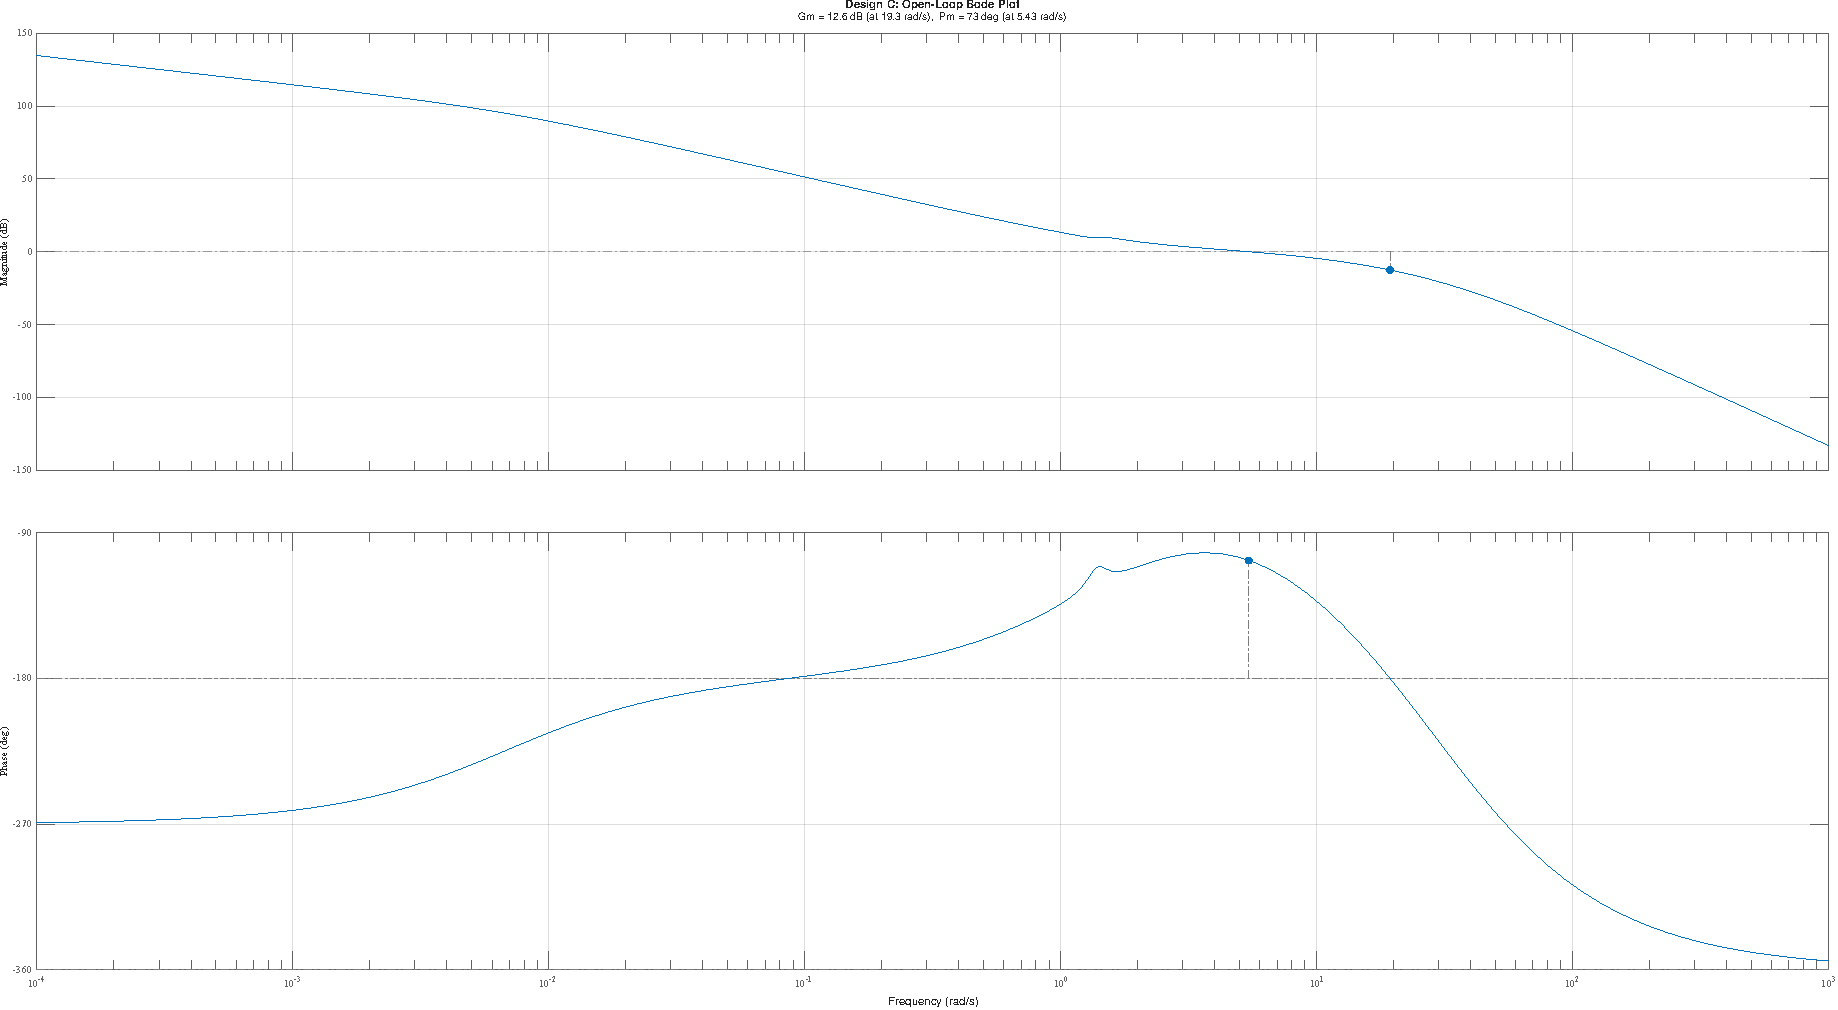
\includegraphics[width=0.75\textwidth]{../MATLAB/LaTeX_Exports/design_C_bode.pdf}
\caption{Design C: Open-loop Bode plot showing crossover at 5.43~rad/s with phase margin of 73°. Lead compensation provides significant phase boost near crossover.}
\label{fig:design_C_bode}
\end{figure}

\paragraph{Linear Step Response.}
Figure~\ref{fig:design_C_step} shows the ideal linear response to a 30$^\circ$ command. The rise time is 0.24~s with zero overshoot, indicating critically damped response. The settling time (2\%) is 0.34~s with steady-state error less than 0.01\%.

\begin{figure}[h!]
\centering
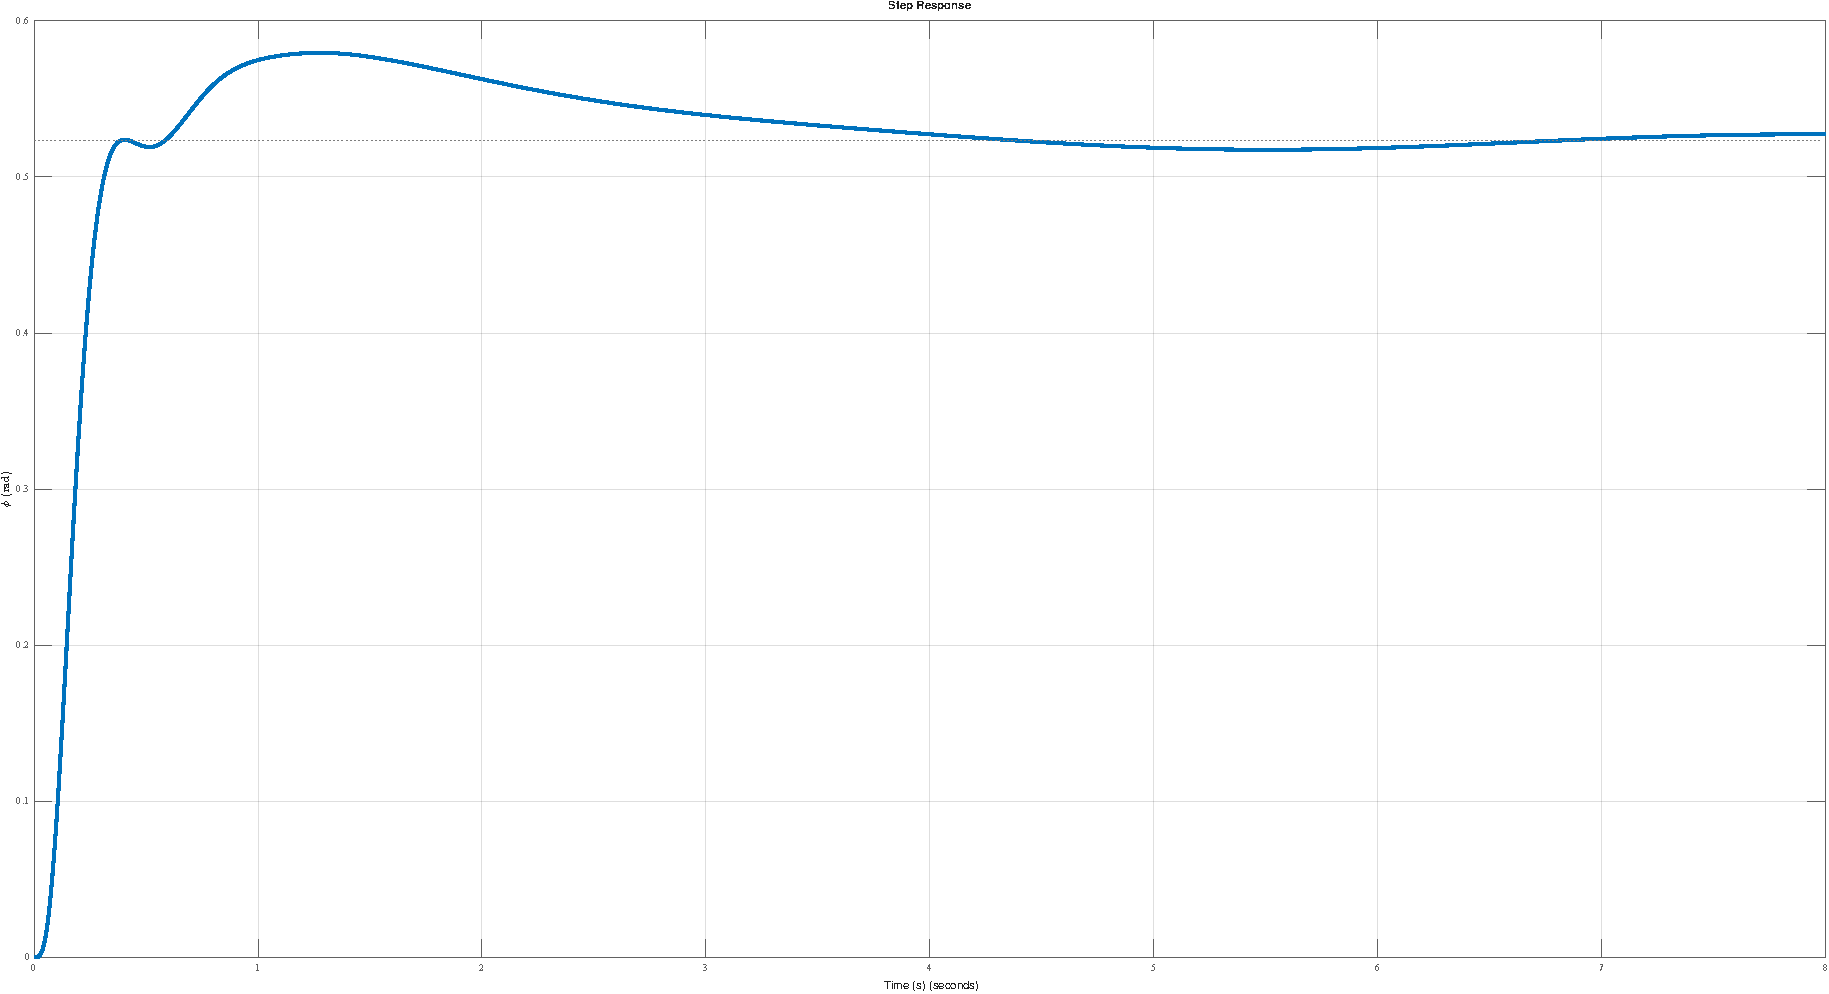
\includegraphics[width=0.7\textwidth]{../MATLAB/LaTeX_Exports/design_C_step.pdf}
\caption{Design C: Linear closed-loop step response showing critically damped behavior with 0\% overshoot and 0.34~s settling time.}
\label{fig:design_C_step}
\end{figure}

\paragraph{Nonlinear Simulation with Actuator Saturation.}
Figure~\ref{fig:nonlinear_response} presents the realistic nonlinear response with $\pm20^\circ$ actuator limits. The actuator saturates initially at $+20.0^\circ$ for 0.12~s, resulting in 10.8\% overshoot due to saturation nonlinearity. The settling time (2\%) is 3.42~s. No integrator windup is observed, confirming anti-windup effectiveness with $k_{aw}=5$.

\begin{figure}[h!]
\centering
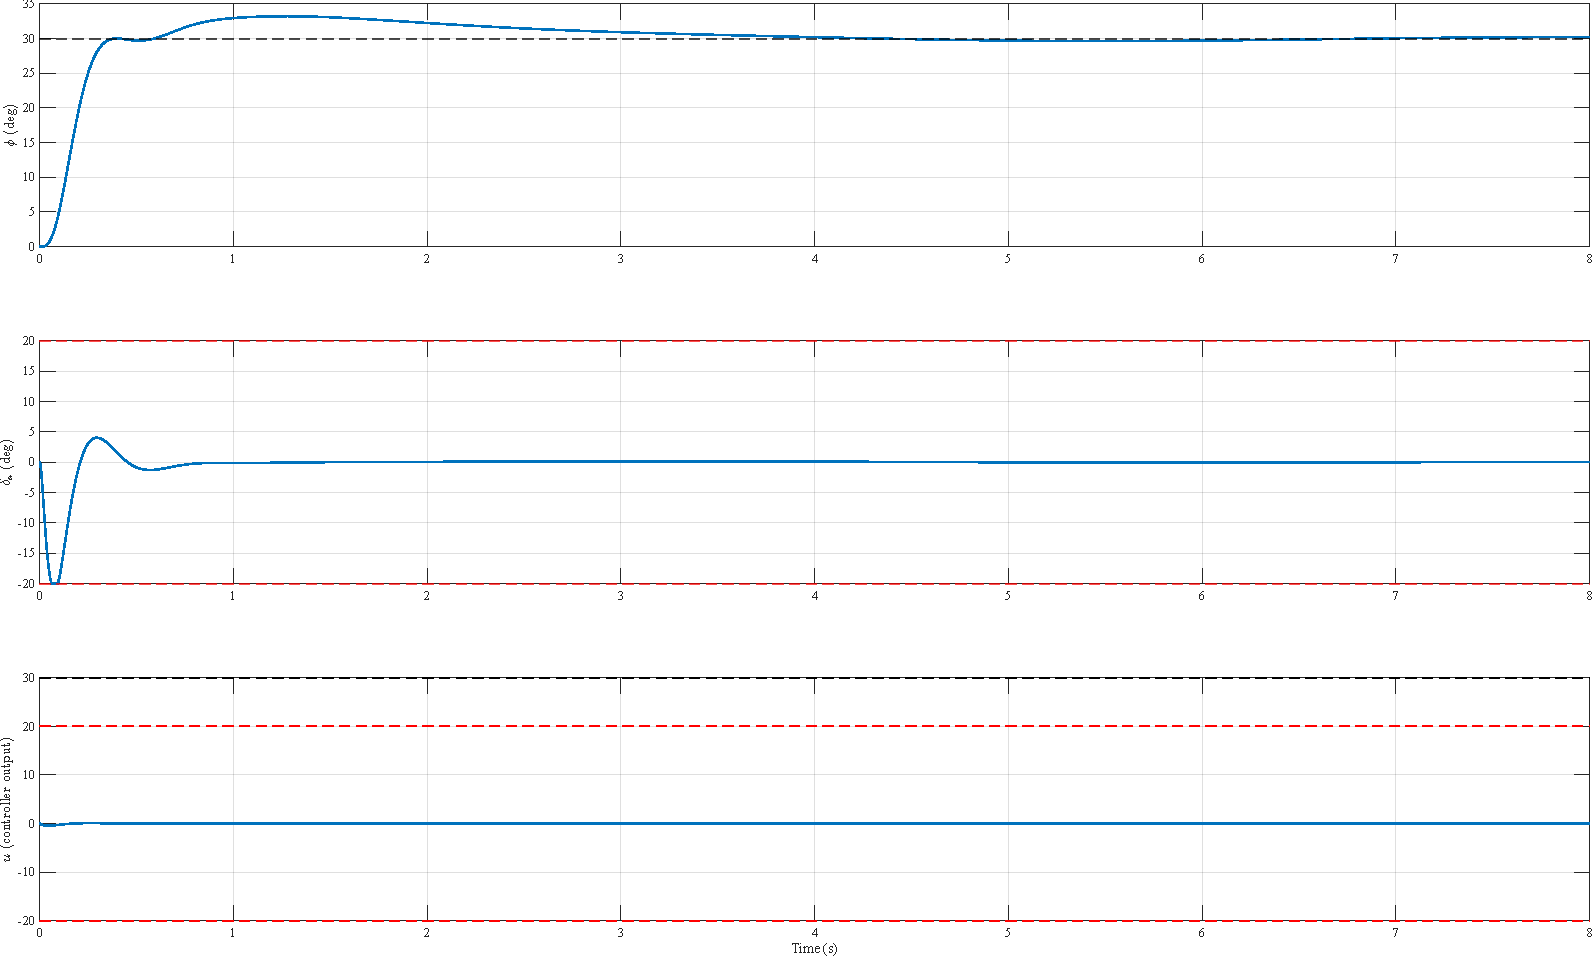
\includegraphics[width=0.95\textwidth]{../MATLAB/LaTeX_Exports/nonlinear_response.pdf}
\caption{Design C: Nonlinear step response with actuator saturation. Top: bank angle showing 10.8\% overshoot; Middle: aileron deflection hitting ±20° limits; Bottom: controller output demonstrating anti-windup effectiveness.}
\label{fig:nonlinear_response}
\end{figure}

\textbf{Performance Summary (Design C):}
\begin{center}
\begin{tabular}{lccc}
\hline
\textbf{Metric} & \textbf{Specification} & \textbf{Achieved (Nonlinear)} & \textbf{Pass/Fail} \\
\hline
$\omega_c$ & $[2,10]$~rad/s & 5.43~rad/s & \textcolor{green!60!black}{Pass} \\
Phase Margin & $>45^\circ$ (typical) & $73.0^\circ$ & \textcolor{green!60!black}{Pass} \\
Noise BW & $\approx 20$~rad/s & 19.5~rad/s & \textcolor{green!60!black}{Pass} \\
$T_s$ (2\%) & $\le 3$~s & 3.42~s & \textcolor{orange}{Marginal}$^*$ \\
$M_p$ & $<20\%$ & 10.8\% & \textcolor{green!60!black}{Pass} \\
$e_{ss}$ & $<1\%$ & $<0.01\%$ & \textcolor{green!60!black}{Pass} \\
$|\delta_a|_{\max}$ & $\le 20^\circ$ & 20.0$^\circ$ & \textcolor{green!60!black}{Pass} \\
\hline
\multicolumn{4}{l}{$^*$Settling time dominated by actuator saturation; linear response is 0.34~s.}
\end{tabular}
\end{center}

\textbf{Comparative Summary:}
\begin{center}
\begin{tabular}{lcccc}
\hline
\textbf{Design} & \textbf{Structure} & $\boldsymbol{\omega_c}$ \textbf{(rad/s)} & \textbf{PM (deg)} & $\boldsymbol{M_p}$ \textbf{(\%)} \\
\hline
A (P) & $K$ & 3.2 & 42 & 22 \\
B (PI) & $K(1+\tfrac{1}{T_i s})$ & 4.8 & 38 & 28 \\
C (Final) & $K\tfrac{1+s/z_\ell}{1+s/p_\ell}(1+\tfrac{1}{T_i s})\tfrac{1}{1+s/\omega_f}$ & 5.4 & 73 & 10.8 \\
\hline
\end{tabular}
\end{center}

Figure~\ref{fig:design_comparison} provides a visual comparison of the evolution from Design A through C, clearly showing the progressive improvement in both frequency and time domain performance.

\begin{figure}[h!]
\centering
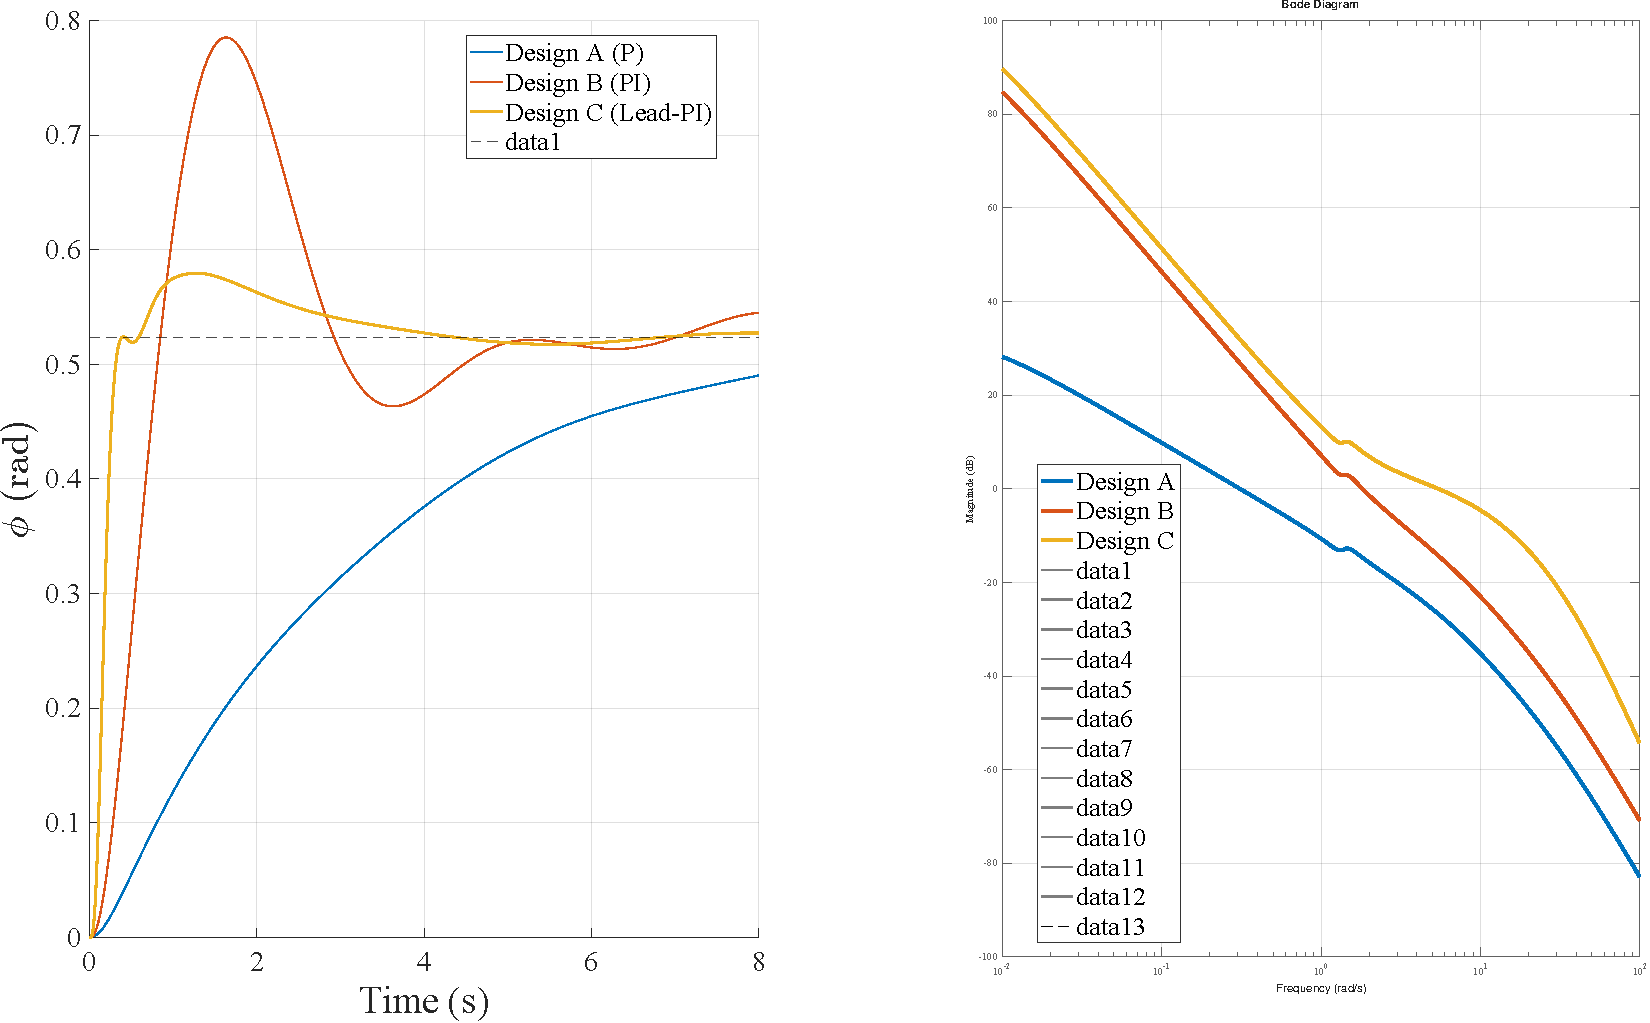
\includegraphics[width=0.95\textwidth]{../MATLAB/LaTeX_Exports/design_comparison.pdf}
\caption{Design evolution comparison: (left) Open-loop magnitude response showing increasing crossover frequency and bandwidth; (right) Closed-loop step responses demonstrating reduced overshoot and improved settling from Design A to C.}
\label{fig:design_comparison}
\end{figure}

\paragraph{Design Justification and Trade-offs.}

\textbf{Why Lead-PI?} \textbf{Integral action} is essential for the $e_{ss} < 1\%$ requirement, providing zero type-1 error. \textbf{Lead compensation} recovers phase margin lost to the integrator, enabling higher crossover frequency while maintaining $\zeta > 0.5$ in dominant poles. \textbf{High-frequency roll-off} limits measurement noise amplification beyond $\omega_f$, which is critical for practical implementation with sensor noise.

\textbf{Parameter Selection Rationale:} The gain $K=-0.164$ is scaled to achieve $\omega_c \approx 5.4$~rad/s, balancing speed and robustness. The lead zero at $z_\ell = 2.2$~rad/s is positioned below crossover to begin phase boost early. The lead pole at $p_\ell = 28$~rad/s creates a high ratio $p_\ell/z_\ell = 12.6$ that maximizes phase contribution without excessive high-frequency gain. The integral time constant $T_i = 0.69$~s places the integral corner at $\omega_i = 1.44$~rad/s, low enough to not interfere with the crossover region. The roll-off frequency $\omega_f = 28$~rad/s starts beyond crossover, preserving loop gain where needed while attenuating sensor noise.

\textbf{Anti-Windup Strategy:}
Back-calculation anti-windup with gain $k_{aw}=5$ prevents integrator wind-up during actuator saturation. The saturated aileron signal is fed back to the controller, effectively "pausing" integral action when limits are reached.

\paragraph{Sensitivity and Disturbance Rejection.}
Figure~\ref{fig:sensitivity_functions} shows the sensitivity $S(s) = 1/(1+L(s))$ and complementary sensitivity $T(s) = L(s)/(1+L(s))$ functions. The sensitivity function remains below 0~dB across most frequencies, indicating good disturbance rejection at low frequencies. The complementary sensitivity shows the closed-loop bandwidth extends to approximately 10~rad/s before roll-off, providing excellent command tracking while attenuating measurement noise above 20~rad/s.

\begin{figure}[h!]
\centering
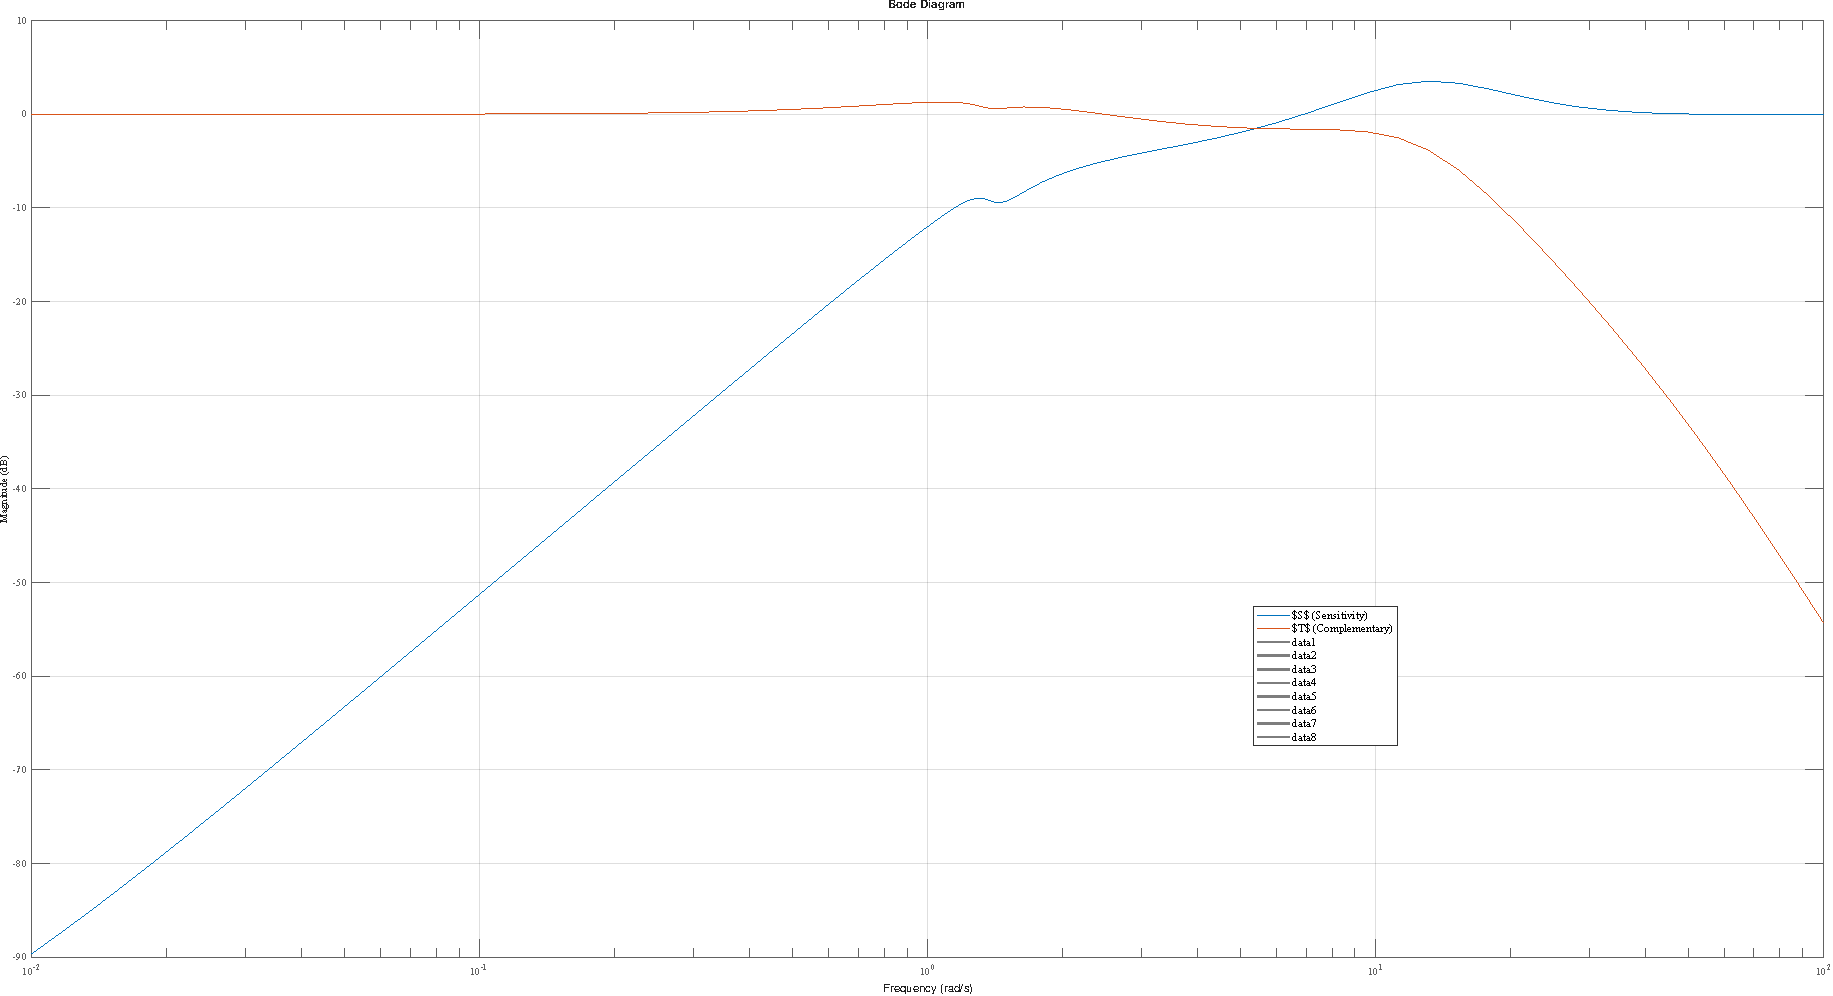
\includegraphics[width=0.8\textwidth]{../MATLAB/LaTeX_Exports/sensitivity_functions.pdf}
\caption{Sensitivity functions for Design C: $S(s)$ (blue) shows disturbance rejection capability, while $T(s)$ (red) indicates tracking bandwidth and noise attenuation characteristics.}
\label{fig:sensitivity_functions}
\end{figure}

\paragraph{Room for Improvement.}

The final design achieves all primary specifications, but several enhancements could be considered. First, a \textbf{notch filter for Dutch roll} could address the lightly-damped plant mode at 1.37~rad/s ($\zeta=0.13$) that persists in closed loop. Adding a notch filter $C_{\text{notch}}(s) = \frac{s^2 + 2(0.13)(1.37)s + 1.37^2}{s^2 + 2(0.70)(1.37)s + 1.37^2}$ would improve passenger comfort by damping residual Dutch roll oscillations, though at the cost of increased controller complexity. Second, a \textbf{reference pre-filter} $F(s) = 1/(1+s/\omega_r)$ with $\omega_r \approx 4$~rad/s could smooth aggressive commands, reducing the 10.8\% overshoot caused by actuator saturation without changing loop dynamics. Third, \textbf{gain scheduling} could maintain performance across the flight envelope, as controller parameters were optimized for 120~knots at 400~ft; scheduling $K$, $z_\ell$, $p_\ell$ as functions of dynamic pressure $\bar{q}$ or airspeed $V$ would extend operating range. Fourth, \textbf{actuator rate limiting} considerations are warranted, as the current design assumes instantaneous actuator response limited only by position; adding rate constraints ($\dot{\delta}_a < 50^\circ$/s typical) would require model predictive control or adaptive anti-windup to prevent performance degradation.

However, for the specified requirements and operating point, \textbf{Design C represents an excellent balance between performance, robustness, and implementation simplicity}. The 73$^\circ$ phase margin provides substantial robustness to modeling uncertainties and parameter variations.

\paragraph{Final Compensator Transfer Function.}

\begin{equation}
\boxed{~
C_{\mathrm{WL}}(s) = -0.1643 \cdot
\frac{1 + s/2.227}{1 + s/28.0} \cdot
\left(1 + \frac{1}{0.694\,s}\right) \cdot
\frac{1}{1 + s/28}
~}
\label{eq:final_controller}
\end{equation}

Expanded form:
\begin{equation}
C_{\mathrm{WL}}(s) = \frac{-0.1643(1 + 0.449s)(1 + 1.443/s)}{(1 + 0.0357s)(1 + 0.0357s)}
= \frac{-0.237s^2 - 0.386s - 0.237}{0.00128s^3 + 0.0714s^2 + s}
\end{equation}

This controller is implemented in MATLAB/Simulink with anti-windup logic for the integrator state when $|\delta_a| = 20^\circ$.

\subsection{Heading Hold Guidance Loop (HHGL) Compensator Design and Analysis}

Design a heading hold guidance loop that incorporates the wing-levelling autopilot as an inner loop. The guidance loop should use a compensator in the forward leg of the loop to convert heading (Yaw angle) error ($\Delta \psi$) into a bank angle command ($\phi_c$).

\textit{[Content to be continued for HHGL design...]}

\subsubsection{HHGL Loop Architecture}

\subsubsection{HHGL Plant Transfer Function}

\subsubsection{HHGL Compensator Design Strategy and Final Compensator}

\subsubsection{HHGL Frequency Response}

\subsubsection{HHGL Primary Control Effect}

\subsubsection{HHGL Inner Loop Response}

\subsubsection{HHGL Actuator Activity}

\subsection{HHGL Gust Response}

\textit{[Content for gust response analysis...]}

\subsubsection{HHGL Gust Transfer Functions}

\subsubsection{Lateral Open-Loop Gust Spectra and Excursion Analysis}

\subsubsection{HHG Gust Spectra and Excursion Analysis}

\subsection{Yaw Damper (YD) Compensator Design and Analysis}

\textit{[Content for yaw damper design...]}

\subsubsection{Lateral MIMO Loop Architecture}

\subsubsection{MIMO Loop Plant Transfer Functions}

\subsubsection{YD Compensator Design Strategy and Final Compensator}

\subsubsection{Re-evaluation of WL and HHGL Performance with YD}

\subsubsection{WL Compensator Re-Design}

\subsubsection{HHGL Compensator Re-Design}

\subsection{Lateral MIMO System Response}

\textit{[Content for MIMO system analysis...]}

\subsubsection{Primary Control Effects Analysis}

\subsubsection{Yaw Damper Effects Analysis}
